\chapter{WF-137 Respecting the Dojo Ratchet To 1965}\label{record-219}

\noindent{\footnotesize\color{BookMuted}\path{docs/design/WF-137-respecting-dojo-ratchet-1965.md}\par}\smallskip

\begin{RecordMeta}
title: WF-137 Respecting the Dojo Ratchet To 1965
legend: WF
lane: bad-code
priority: high
github_issue: 379
status: complete
keywords:
  - code-dojo
  - eslint
  - standards
  - ratchet
  - respectful-repo

\end{RecordMeta}

Legend: \href{https://github.com/flyingrobots/bijou/blob/cbd70612140e7a450d764b3c7be1c6af878b99bc/docs/legends/WF-workflow-delivery.md}{WF - Workflow and Delivery}

\section{Linked Work}\label{record-219-linked-work}

\begin{itemize}
\tightlist
\item
  Issue: \href{https://github.com/flyingrobots/bijou/issues/379}{\#379}
\item
  Standards artifact: \href{https://github.com/flyingrobots/bijou/blob/cbd70612140e7a450d764b3c7be1c6af878b99bc/docs/typescript-code-standards.editors-edition.md}{TypeScript Code Standards Editor's Edition}
\item
  Exception ledger: \href{https://github.com/flyingrobots/bijou/blob/cbd70612140e7a450d764b3c7be1c6af878b99bc/docs/code-dojo-exceptions.md}{Code Dojo Exceptions}
\end{itemize}

\section{Decision Summary}\label{record-219-decision-summary}

WF-136 merged with aggregate Code Dojo debt at \texttt{2\allowbreak{},\allowbreak{}0\allowbreak{}1\allowbreak{}5}, including \texttt{1\allowbreak{},\allowbreak{}6\allowbreak{}0\allowbreak{}3} type-aware ESLint findings. The repo goal remains zero ESLint errors, zero Code Dojo issues, and zero files violating length restrictions. The ratchet policy requires every met goalpost to remove at least 50 counted violations until zero.

This cycle targets the next ratchet: lower aggregate debt from \texttt{2\allowbreak{},\allowbreak{}0\allowbreak{}1\allowbreak{}5} to \texttt{1\allowbreak{},\allowbreak{}9\allowbreak{}6\allowbreak{}5} or lower without weakening rules, excluding files, or raising any baseline.

\section{Sponsored Human}\label{record-219-sponsored-human}

A maintainer wants the post-merge Dojo loop to keep moving while the next target is fresh and the local iteration path is still warm.

\section{Sponsored Agent}\label{record-219-sponsored-agent}

An agent needs a small, non-DOGFOOD cleanup cluster that clears the next 50-count ratchet without pulling the localization debt gate into unrelated source edits.

\section{Hill}\label{record-219-hill}

Reduce aggregate Code Dojo debt from \texttt{2\allowbreak{},\allowbreak{}0\allowbreak{}1\allowbreak{}5} to \texttt{1\allowbreak{},\allowbreak{}9\allowbreak{}6\allowbreak{}5} or lower by eliminating at least \texttt{5\allowbreak{}0} live ESLint findings from non-DOGFOOD package or test files.

Current candidates from the offender list:

\begin{center}
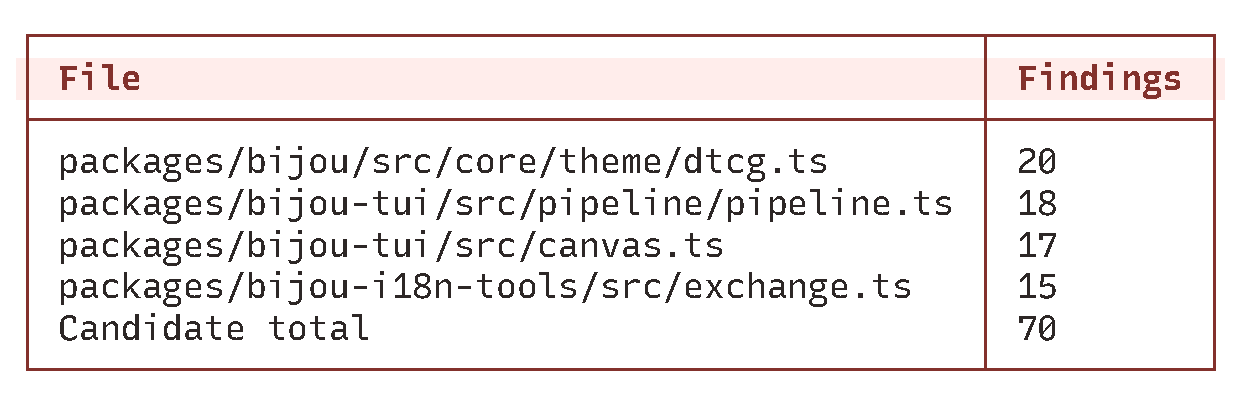
\includegraphics[width=\linewidth]{figures/tables/table-047-g1-1.pdf}
\par\smallskip{\scriptsize\color{BookMuted}Rows 1–5. Actual Bijou table component.}
\end{center}


The final slice may substitute equivalent non-DOGFOOD files if a candidate would require broader semantic work than the goalpost warrants.

\section{Scope}\label{record-219-scope}

\begin{itemize}
\tightlist
\item
  Replace unsafe theme-token and pipeline assertions with explicit guards or narrower local types.
\item
  Replace assertion-based array/object reads with checked reads or direct value iteration.
\item
  Make template interpolation explicit where values are not statically strings.
\item
  Keep rendering, pipeline, and i18n exchange behavior stable.
\item
  Lower \texttt{s\allowbreak{}c\allowbreak{}r\allowbreak{}i\allowbreak{}p\allowbreak{}t\allowbreak{}s\allowbreak{}/\allowbreak{}c\allowbreak{}o\allowbreak{}d\allowbreak{}e\allowbreak{}-\allowbreak{}d\allowbreak{}o\allowbreak{}j\allowbreak{}o\allowbreak{}/\allowbreak{}b\allowbreak{}a\allowbreak{}s\allowbreak{}e\allowbreak{}l\allowbreak{}i\allowbreak{}n\allowbreak{}e\allowbreak{}s\allowbreak{}/\allowbreak{}e\allowbreak{}s\allowbreak{}l\allowbreak{}i\allowbreak{}n\allowbreak{}t\allowbreak{}.\allowbreak{}j\allowbreak{}s\allowbreak{}o\allowbreak{}n}, \texttt{d\allowbreak{}o\allowbreak{}c\allowbreak{}s\allowbreak{}/\allowbreak{}c\allowbreak{}o\allowbreak{}d\allowbreak{}e\allowbreak{}-\allowbreak{}d\allowbreak{}o\allowbreak{}j\allowbreak{}o\allowbreak{}-\allowbreak{}e\allowbreak{}x\allowbreak{}c\allowbreak{}e\allowbreak{}p\allowbreak{}t\allowbreak{}i\allowbreak{}o\allowbreak{}n\allowbreak{}s\allowbreak{}.\allowbreak{}m\allowbreak{}d}, and \texttt{p\allowbreak{}a\allowbreak{}c\allowbreak{}k\allowbreak{}a\allowbreak{}g\allowbreak{}e\allowbreak{}.\allowbreak{}j\allowbreak{}s\allowbreak{}o\allowbreak{}n} only after live counts prove the reduction.
\end{itemize}

\section{Non-Goals}\label{record-219-non-goals}

\begin{itemize}
\tightlist
\item
  Leave the 5,000-line DOGFOOD app untouched in this slice.
\item
  Keep ESLint rules and Code Dojo thresholds at full strength.
\item
  Preserve file/context and code-size ceilings.
\item
  Avoid architectural rewrites outside the selected cleanup files.
\end{itemize}

\section{Current Evidence}\label{record-219-current-evidence}

Live counts on \texttt{m\allowbreak{}a\allowbreak{}i\allowbreak{}n} at \texttt{e\allowbreak{}6\allowbreak{}c\allowbreak{}8\allowbreak{}b\allowbreak{}d\allowbreak{}d\allowbreak{}1}:

\begin{itemize}
\tightlist
\item
  aggregate Code Dojo debt: \texttt{2\allowbreak{},\allowbreak{}0\allowbreak{}1\allowbreak{}5}
\item
  ESLint findings: \texttt{1\allowbreak{},\allowbreak{}6\allowbreak{}0\allowbreak{}3}
\item
  file/context baseline: \texttt{3\allowbreak{}3\allowbreak{}3}
\item
  mock-ban baseline: \texttt{2\allowbreak{}3}
\item
  code-size baseline: \texttt{5\allowbreak{}6}, including \texttt{4} legacy hard-limit files
\item
  next aggregate target: \texttt{1\allowbreak{},\allowbreak{}9\allowbreak{}6\allowbreak{}5} or lower
\end{itemize}

\section{Playback Questions}\label{record-219-playback-questions}

\begin{enumerate}
\def\labelenumi{\arabic{enumi}.}
\tightlist
\item
  Is aggregate Code Dojo debt at \texttt{1\allowbreak{},\allowbreak{}9\allowbreak{}6\allowbreak{}5} or lower?
\item
  Does the stored ESLint baseline match the new live count?
\item
  Have file/context and code-size debt held or shrunk?
\item
  Do focused tests for the touched surfaces pass?
\item
  Are the repo gates passing before review?
\end{enumerate}

\section{Tests To Write First}\label{record-219-tests-to-write-first}

The lint findings are the RED signal for pure type-safety rewrites. Add focused regression tests before changing rendering, pipeline execution, or i18n exchange behavior.

\section{Acceptance Criteria}\label{record-219-acceptance-criteria}

\begin{itemize}
\tightlist
\item
  The selected touched TypeScript files have zero new ESLint findings and reduce live findings by at least \texttt{5\allowbreak{}0}.
\item
  Aggregate Code Dojo debt is \texttt{1\allowbreak{},\allowbreak{}9\allowbreak{}6\allowbreak{}5} or lower.
\item
  \texttt{s\allowbreak{}c\allowbreak{}r\allowbreak{}i\allowbreak{}p\allowbreak{}t\allowbreak{}s\allowbreak{}/\allowbreak{}c\allowbreak{}o\allowbreak{}d\allowbreak{}e\allowbreak{}-\allowbreak{}d\allowbreak{}o\allowbreak{}j\allowbreak{}o\allowbreak{}/\allowbreak{}b\allowbreak{}a\allowbreak{}s\allowbreak{}e\allowbreak{}l\allowbreak{}i\allowbreak{}n\allowbreak{}e\allowbreak{}s\allowbreak{}/\allowbreak{}e\allowbreak{}s\allowbreak{}l\allowbreak{}i\allowbreak{}n\allowbreak{}t\allowbreak{}.\allowbreak{}j\allowbreak{}s\allowbreak{}o\allowbreak{}n} records the lower live ESLint count.
\item
  \texttt{d\allowbreak{}o\allowbreak{}c\allowbreak{}s\allowbreak{}/\allowbreak{}c\allowbreak{}o\allowbreak{}d\allowbreak{}e\allowbreak{}-\allowbreak{}d\allowbreak{}o\allowbreak{}j\allowbreak{}o\allowbreak{}-\allowbreak{}e\allowbreak{}x\allowbreak{}c\allowbreak{}e\allowbreak{}p\allowbreak{}t\allowbreak{}i\allowbreak{}o\allowbreak{}n\allowbreak{}s\allowbreak{}.\allowbreak{}m\allowbreak{}d} and \texttt{p\allowbreak{}a\allowbreak{}c\allowbreak{}k\allowbreak{}a\allowbreak{}g\allowbreak{}e\allowbreak{}.\allowbreak{}j\allowbreak{}s\allowbreak{}o\allowbreak{}n} report the lower ceiling.
\item
  Focused validation for the touched surfaces passes.
\item
  \texttt{n\allowbreak{}p\allowbreak{}m\allowbreak{} \allowbreak{}r\allowbreak{}u\allowbreak{}n\allowbreak{} \allowbreak{}c\allowbreak{}o\allowbreak{}d\allowbreak{}e\allowbreak{}-\allowbreak{}d\allowbreak{}o\allowbreak{}j\allowbreak{}o\allowbreak{}:\allowbreak{}v\allowbreak{}e\allowbreak{}r\allowbreak{}i\allowbreak{}f\allowbreak{}y}, \texttt{n\allowbreak{}p\allowbreak{}m\allowbreak{} \allowbreak{}r\allowbreak{}u\allowbreak{}n\allowbreak{} \allowbreak{}d\allowbreak{}o\allowbreak{}c\allowbreak{}s\allowbreak{}:\allowbreak{}i\allowbreak{}n\allowbreak{}v\allowbreak{}e\allowbreak{}n\allowbreak{}t\allowbreak{}o\allowbreak{}r\allowbreak{}y}, \texttt{n\allowbreak{}p\allowbreak{}m\allowbreak{} \allowbreak{}r\allowbreak{}u\allowbreak{}n\allowbreak{} \allowbreak{}l\allowbreak{}i\allowbreak{}n\allowbreak{}t}, and \texttt{g\allowbreak{}i\allowbreak{}t\allowbreak{} \allowbreak{}d\allowbreak{}i\allowbreak{}f\allowbreak{}f\allowbreak{} \allowbreak{}-\allowbreak{}-\allowbreak{}c\allowbreak{}h\allowbreak{}e\allowbreak{}c\allowbreak{}k} pass before review.
\end{itemize}

\section{Retrospective}\label{record-219-retrospective}

Completed with aggregate Code Dojo debt reduced from \texttt{2\allowbreak{},\allowbreak{}0\allowbreak{}1\allowbreak{}5} to \texttt{1\allowbreak{},\allowbreak{}9\allowbreak{}0\allowbreak{}7} (\texttt{-\allowbreak{}1\allowbreak{}0\allowbreak{}8}). The stored ESLint baseline now records \texttt{1\allowbreak{},\allowbreak{}4\allowbreak{}9\allowbreak{}5} live findings, down from \texttt{1\allowbreak{},\allowbreak{}6\allowbreak{}0\allowbreak{}3}, and the next aggregate target is \texttt{1\allowbreak{},\allowbreak{}8\allowbreak{}5\allowbreak{}7} or lower.

The implementation cleaned six non-DOGFOOD files:

\begin{itemize}
\tightlist
\item
  \texttt{p\allowbreak{}a\allowbreak{}c\allowbreak{}k\allowbreak{}a\allowbreak{}g\allowbreak{}e\allowbreak{}s\allowbreak{}/\allowbreak{}b\allowbreak{}i\allowbreak{}j\allowbreak{}o\allowbreak{}u\allowbreak{}/\allowbreak{}s\allowbreak{}r\allowbreak{}c\allowbreak{}/\allowbreak{}c\allowbreak{}o\allowbreak{}r\allowbreak{}e\allowbreak{}/\allowbreak{}t\allowbreak{}h\allowbreak{}e\allowbreak{}m\allowbreak{}e\allowbreak{}/\allowbreak{}d\allowbreak{}t\allowbreak{}c\allowbreak{}g\allowbreak{}.\allowbreak{}t\allowbreak{}s} now treats imported DTCG documents as unknown-shaped records and validates token, modifier, RGB, group, and JSON reads locally instead of casting external payloads into narrower types.
\item
  \texttt{p\allowbreak{}a\allowbreak{}c\allowbreak{}k\allowbreak{}a\allowbreak{}g\allowbreak{}e\allowbreak{}s\allowbreak{}/\allowbreak{}b\allowbreak{}i\allowbreak{}j\allowbreak{}o\allowbreak{}u\allowbreak{}-\allowbreak{}t\allowbreak{}u\allowbreak{}i\allowbreak{}/\allowbreak{}s\allowbreak{}r\allowbreak{}c\allowbreak{}/\allowbreak{}c\allowbreak{}a\allowbreak{}n\allowbreak{}v\allowbreak{}a\allowbreak{}s\allowbreak{}.\allowbreak{}t\allowbreak{}s} now uses \texttt{u\allowbreak{}n\allowbreak{}k\allowbreak{}n\allowbreak{}o\allowbreak{}w\allowbreak{}n} shader uniforms, preserves packed-surface narrowing directly, computes UV denominators explicitly, and removes assertion-based Braille dot reads.
\item
  \texttt{p\allowbreak{}a\allowbreak{}c\allowbreak{}k\allowbreak{}a\allowbreak{}g\allowbreak{}e\allowbreak{}s\allowbreak{}/\allowbreak{}b\allowbreak{}i\allowbreak{}j\allowbreak{}o\allowbreak{}u\allowbreak{}-\allowbreak{}i\allowbreak{}1\allowbreak{}8\allowbreak{}n\allowbreak{}-\allowbreak{}t\allowbreak{}o\allowbreak{}o\allowbreak{}l\allowbreak{}s\allowbreak{}/\allowbreak{}s\allowbreak{}r\allowbreak{}c\allowbreak{}/\allowbreak{}e\allowbreak{}x\allowbreak{}c\allowbreak{}h\allowbreak{}a\allowbreak{}n\allowbreak{}g\allowbreak{}e\allowbreak{}.\allowbreak{}t\allowbreak{}s} now validates serialized exchange value kinds before decoding, validates external collection arrays before iterating, keeps external version fields checkable, and derives workbook row typing from the column manifest.
\item
  \texttt{p\allowbreak{}a\allowbreak{}c\allowbreak{}k\allowbreak{}a\allowbreak{}g\allowbreak{}e\allowbreak{}s\allowbreak{}/\allowbreak{}b\allowbreak{}i\allowbreak{}j\allowbreak{}o\allowbreak{}u\allowbreak{}/\allowbreak{}s\allowbreak{}r\allowbreak{}c\allowbreak{}/\allowbreak{}f\allowbreak{}a\allowbreak{}c\allowbreak{}t\allowbreak{}o\allowbreak{}r\allowbreak{}y\allowbreak{}.\allowbreak{}t\allowbreak{}s} now shares the DTCG JSON document guard used by file-based theme loading instead of asserting parsed environment payloads.
\item
  \texttt{p\allowbreak{}a\allowbreak{}c\allowbreak{}k\allowbreak{}a\allowbreak{}g\allowbreak{}e\allowbreak{}s\allowbreak{}/\allowbreak{}b\allowbreak{}i\allowbreak{}j\allowbreak{}o\allowbreak{}u\allowbreak{}-\allowbreak{}t\allowbreak{}u\allowbreak{}i\allowbreak{}/\allowbreak{}s\allowbreak{}r\allowbreak{}c\allowbreak{}/\allowbreak{}o\allowbreak{}v\allowbreak{}e\allowbreak{}r\allowbreak{}l\allowbreak{}a\allowbreak{}y\allowbreak{}.\allowbreak{}t\allowbreak{}s} now guards resolved color records and packed-buffer reads without non-null assertions while preserving drawer and inherited-background behavior.
\item
  \texttt{p\allowbreak{}a\allowbreak{}c\allowbreak{}k\allowbreak{}a\allowbreak{}g\allowbreak{}e\allowbreak{}s\allowbreak{}/\allowbreak{}b\allowbreak{}i\allowbreak{}j\allowbreak{}o\allowbreak{}u\allowbreak{}-\allowbreak{}t\allowbreak{}u\allowbreak{}i\allowbreak{}/\allowbreak{}s\allowbreak{}r\allowbreak{}c\allowbreak{}/\allowbreak{}p\allowbreak{}i\allowbreak{}p\allowbreak{}e\allowbreak{}l\allowbreak{}i\allowbreak{}n\allowbreak{}e\allowbreak{}/\allowbreak{}p\allowbreak{}i\allowbreak{}p\allowbreak{}e\allowbreak{}l\allowbreak{}i\allowbreak{}n\allowbreak{}e\allowbreak{}.\allowbreak{}t\allowbreak{}s} now uses \texttt{u\allowbreak{}n\allowbreak{}k\allowbreak{}n\allowbreak{}o\allowbreak{}w\allowbreak{}n} render-state extension data, guarded layout-root and thenable reads, explicit unknown error formatting, and preserved halted-stage timing semantics.
\item
  \texttt{p\allowbreak{}a\allowbreak{}c\allowbreak{}k\allowbreak{}a\allowbreak{}g\allowbreak{}e\allowbreak{}s\allowbreak{}/\allowbreak{}b\allowbreak{}i\allowbreak{}j\allowbreak{}o\allowbreak{}u\allowbreak{}-\allowbreak{}t\allowbreak{}u\allowbreak{}i\allowbreak{}/\allowbreak{}s\allowbreak{}r\allowbreak{}c\allowbreak{}/\allowbreak{}r\allowbreak{}u\allowbreak{}n\allowbreak{}t\allowbreak{}i\allowbreak{}m\allowbreak{}e\allowbreak{}.\allowbreak{}t\allowbreak{}s} now avoids \texttt{v\allowbreak{}o\allowbreak{}i\allowbreak{}d} unions in lifecycle hook returns, keeps render/crash queue checks explicit, removes the legacy \texttt{l\allowbreak{}a\allowbreak{}y\allowbreak{}o\allowbreak{}u\allowbreak{}t\allowbreak{}R\allowbreak{}o\allowbreak{}o\allowbreak{}t} mutation, and formats runtime errors without object stringification.
\end{itemize}

Touched file/context budgets held or shrank: \texttt{d\allowbreak{}t\allowbreak{}c\allowbreak{}g\allowbreak{}.\allowbreak{}t\allowbreak{}s} is now \texttt{3\allowbreak{}1\allowbreak{}4} lines / \texttt{1\allowbreak{}0\allowbreak{},\allowbreak{}4\allowbreak{}9\allowbreak{}1} bytes against a \texttt{3\allowbreak{}4\allowbreak{}7} / \texttt{1\allowbreak{}2\allowbreak{},\allowbreak{}3\allowbreak{}4\allowbreak{}6} baseline, \texttt{c\allowbreak{}a\allowbreak{}n\allowbreak{}v\allowbreak{}a\allowbreak{}s\allowbreak{}.\allowbreak{}t\allowbreak{}s} is now \texttt{3\allowbreak{}5\allowbreak{}8} lines / \texttt{1\allowbreak{}0\allowbreak{},\allowbreak{}9\allowbreak{}5\allowbreak{}3} bytes against a \texttt{3\allowbreak{}7\allowbreak{}7} / \texttt{1\allowbreak{}1\allowbreak{},\allowbreak{}2\allowbreak{}9\allowbreak{}5} baseline, and \texttt{e\allowbreak{}x\allowbreak{}c\allowbreak{}h\allowbreak{}a\allowbreak{}n\allowbreak{}g\allowbreak{}e\allowbreak{}.\allowbreak{}t\allowbreak{}s} is now \texttt{3\allowbreak{}5\allowbreak{}6} lines / \texttt{1\allowbreak{}1\allowbreak{},\allowbreak{}3\allowbreak{}9\allowbreak{}0} bytes against a \texttt{3\allowbreak{}6\allowbreak{}1} / \texttt{1\allowbreak{}1\allowbreak{},\allowbreak{}4\allowbreak{}5\allowbreak{}9} baseline. The follow-on TUI slice held the same ratchet: \texttt{o\allowbreak{}v\allowbreak{}e\allowbreak{}r\allowbreak{}l\allowbreak{}a\allowbreak{}y\allowbreak{}.\allowbreak{}t\allowbreak{}s} is now \texttt{9\allowbreak{}3\allowbreak{}3} lines / \texttt{3\allowbreak{}3\allowbreak{},\allowbreak{}3\allowbreak{}3\allowbreak{}2} bytes against a \texttt{9\allowbreak{}4\allowbreak{}2} / \texttt{3\allowbreak{}3\allowbreak{},\allowbreak{}7\allowbreak{}2\allowbreak{}1} baseline, \texttt{p\allowbreak{}i\allowbreak{}p\allowbreak{}e\allowbreak{}l\allowbreak{}i\allowbreak{}n\allowbreak{}e\allowbreak{}.\allowbreak{}t\allowbreak{}s} is now \texttt{2\allowbreak{}3\allowbreak{}8} lines / \texttt{7\allowbreak{},\allowbreak{}7\allowbreak{}5\allowbreak{}6} bytes against a \texttt{2\allowbreak{}6\allowbreak{}8} / \texttt{8\allowbreak{},\allowbreak{}6\allowbreak{}4\allowbreak{}6} baseline, and \texttt{r\allowbreak{}u\allowbreak{}n\allowbreak{}t\allowbreak{}i\allowbreak{}m\allowbreak{}e\allowbreak{}.\allowbreak{}t\allowbreak{}s} is now \texttt{6\allowbreak{}6\allowbreak{}9} lines / \texttt{1\allowbreak{}9\allowbreak{},\allowbreak{}4\allowbreak{}9\allowbreak{}1} bytes against a \texttt{6\allowbreak{}9\allowbreak{}5} / \texttt{2\allowbreak{}0\allowbreak{},\allowbreak{}6\allowbreak{}4\allowbreak{}0} baseline.

